\documentclass[xcolor={dvipsnames}]{beamer}
%\usepackage[utf8]{inputenc}
\usetheme{Madrid}
%\usetheme{Malmoe}
\usecolortheme{beaver}
%\usecolortheme{rose}

%-------------------------------------------------------------------------------
%          -Packages nécessaires pour écrire en Français et en UTF8-
%-------------------------------------------------------------------------------
\usepackage[utf8]{inputenc}
\usepackage[frenchb]{babel}
\usepackage[T1]{fontenc}
\usepackage{lmodern}
\usepackage{textcomp}

%-------------------------------------------------------------------------------

%-------------------------------------------------------------------------------
%                          -Outils de mise en forme-
%-------------------------------------------------------------------------------
\usepackage{hyperref}
\hypersetup{pdfstartview=XYZ}
\usepackage{enumerate}
\usepackage{graphicx}
%\usepackage{multicol}
%\usepackage{tabularx}

%\usepackage{anysize} %%pour pouvoir mettre les marges qu'on veut
%\marginsize{2.5cm}{2.5cm}{2.5cm}{2.5cm}

\usepackage{indentfirst} %%pour que les premier paragraphes soient aussi indentés
\usepackage{verbatim}
%\usepackage[table]{xcolor}  
%\usepackage{multirow}
\usepackage{ulem}
%-------------------------------------------------------------------------------


%-------------------------------------------------------------------------------
%                  -Nécessaires pour écrire des mathématiques-
%-------------------------------------------------------------------------------
\usepackage{amsfonts}
\usepackage{amssymb}
\usepackage{amsmath}
\usepackage{amsthm}
\usepackage{tikz}
\usepackage{xlop}
\usepackage[output-decimal-marker={,}]{siunitx}
%-------------------------------------------------------------------------------


%-------------------------------------------------------------------------------
%                    - Mise en forme 
%-------------------------------------------------------------------------------

\newcommand{\bu}[1]{\underline{\textbf{#1}}}


\usepackage{ifthen}


\newcommand{\ifTrue}[2]{\ifthenelse{\equal{#1}{true}}{#2}{$\qquad \qquad$}}

\newcommand{\kword}[1]{\textcolor{red}{\underline{#1}}}


%-------------------------------------------------------------------------------



%-------------------------------------------------------------------------------
%                    - Racourcis d'écriture -
%-------------------------------------------------------------------------------

% Angles orientés (couples de vecteurs)
\newcommand{\aopp}[2]{(\vec{#1}, \vec{#2})} %Les deuc vecteurs sont positifs
\newcommand{\aopn}[2]{(\vec{#1}, -\vec{#2})} %Le second vecteur est négatif
\newcommand{\aonp}[2]{(-\vec{#1}, \vec{#2})} %Le premier vecteur est négatif
\newcommand{\aonn}[2]{(-\vec{#1}, -\vec{#2})} %Les deux vecteurs sont négatifs

%Ensembles mathématiques
\newcommand{\naturels}{\mathbb{N}} %Nombres naturels
\newcommand{\relatifs}{\mathbb{Z}} %Nombres relatifs
\newcommand{\rationnels}{\mathbb{Q}} %Nombres rationnels
\newcommand{\reels}{\mathbb{R}} %Nombres réels
\newcommand{\complexes}{\mathbb{C}} %Nombres complexes


%Intégration des parenthèses aux cosinus
\newcommand{\cosP}[1]{\cos\left(#1\right)}
\newcommand{\sinP}[1]{\sin\left(#1\right)}

%Fractions
\newcommand{\myfrac}[2]{{\LARGE $\frac{#1}{#2}$}}

%Vocabulaire courrant
\newcommand{\cad}{c'est-à-dire}

%Droites
\newcommand{\dte}[1]{droite $(#1)$}
\newcommand{\fig}[1]{figure $#1$}
\newcommand{\sym}{symétrique}
\newcommand{\syms}{symétriques}
\newcommand{\asym}{axe de symétrie}
\newcommand{\asyms}{axes de symétrie}
\newcommand{\seg}[1]{$[#1]$}
\newcommand{\monAngle}[1]{$\widehat{#1}$}
\newcommand{\bissec}{bissectrice}
\newcommand{\mediat}{médiatrice}
\newcommand{\ddte}[1]{$[#1)$}

%Figures
\newcommand{\para}{parallélogramme}
\newcommand{\paras}{parallélogrammes}
\newcommand{\myquad}{quadrilatère}
\newcommand{\myquads}{quadrilatères}
\newcommand{\co}{côtés opposés}
\newcommand{\diag}{diagonale}
\newcommand{\diags}{diagonales}
\newcommand{\supp}{supplémentaires}
\newcommand{\car}{carré}
\newcommand{\cars}{carrés}
\newcommand{\rect}{rectangle}
\newcommand{\rects}{rectangles}
\newcommand{\los}{losange}
\newcommand{\loss}{losanges}


%----------------------------------------------------


\usepackage{../../../../pas-math}
\usepackage{../../../../moncours_beamer}

\usepackage{amssymb,amsmath}


\newcommand{\myitem}{\item[\textbullet]}

\graphicspath{{../img/}}

\title{Chapitre 1 : Nombre entiers et décimaux}
%\author{O. FINOT}\institute{Collège S$^t$ Bernard}

%
\AtBeginSection[]
{
	\begin{frame}
		\frametitle{}
		\tableofcontents[currentsection, hideallsubsections]
	\end{frame} 

}
%
%
%\AtBeginSubsection[]
%{
%	\begin{frame}
%		\frametitle{Sommaire}
%		\tableofcontents[currentsection, currentsubsection]
%	\end{frame} 
%}

\begin{document}



\begin{frame}
  \titlepage 
\end{frame}


	
\begin{frame}
	\begin{block}{Objectifs}
		Savoir :
		\begin{itemize}
			
			\item  écrire des nombres en chiffres et en toutes lettres;
			\item décomposer un nombre;
			\item comparer et ranger des nombres;
			\item  encadrer un nombre ;
			\item placer un nombre sur une demi-droite graduée et lire une abscisse.\pause
		\end{itemize}
	\end{block}


	\begin{block}{Compétence}
		\textbf{Représenter} :
		produire et utiliser diverses représentations des fractions simples et des nombres décimaux .
	\end{block}
\end{frame}


\section{\'Ecrire un nombre}




\begin{frame}{}

	\begin{block}{Activité 1 Différentes écritures d'un nombre}
		\begin{enumerate}\pause
			\item 
			\begin{itemize}
				\item 17 et 42 sont des nombres à 2 chiffres;\pause
				\item 128 et 512 sont des nombres à 3 chiffres;\pause
				\item \num{2048} et \num{4096} sont des nombres à 4 chiffres;\pause
				\item \num{16384} et \num{65536} sont des nombres à 5 chiffres.\pause
			\end{itemize}
			
			%\item \'Ecrire les nombres suivants en toutes lettres : \num{32}, \num{128} et \num{1024}. 
			\item Le nombre 25146041337 s'écrit \num{25146041337}.\pause
			\item 
			\begin{itemize}
				\item 3,4 milliers s'écrit \num{3400};\pause
				\item 144,8 millions s'écrit \num{144800000};\pause
				\item 163 milliards s'écrit \num{163000000000}.\pause
			\end{itemize}
			
			\item .
			\begin{itemize}
				\item Cinq-cent-un-millions-six-cent-vingt-deux-mille-sept-cent-trente-et-un s'écrit \num{501622731};\pause
				\item Cinq-cent-millions s'écrit \num{500000000}.\pause
			\end{itemize}
			
		\end{enumerate}
	\end{block}
\end{frame}



\begin{frame}
	\begin{alertblock}{Définitions}
		\begin{itemize}\pause
			\item Il existe 10 \kword{chiffres} : \pause 0, 1, 2, 3, 4, 5, 6, 7, 8 et 9.\pause
			
			\item On utilise les chiffres pour \pause écrire des \kword{nombres}.\pause	
		
		\end{itemize}
	\end{alertblock}

	\begin{exampleblock}{Exemples}
		\begin{enumerate}
			\item Quels nombres peut-on écrire uniquement avec les chiffres  2 et 4 ?\pause
			
			On peut écrire les nombres 24 et 42. \pause
			\item Le nombre \num{49096} s'écrit avec quels chiffres ? \pause 
			Il s'écrit avec les chiffres 4, 0, 9 et 6.
			
		\end{enumerate}
	\end{exampleblock}

	
\end{frame}



\begin{frame}
	\begin{alertblock}{Définitions}
		\begin{itemize}\pause
			\item Pour mieux lire un grand nombre, on regroupe \pause ses chiffres en classes par groupe de 3.\pause
			
			\item Un \kw{nombre décimal} possède \pause une \kw{partie entière} (avant la virgule) et une \kw{partie décimale} (après la virgule).\pause
			
			\item Un \kw{nombre entier} est un nombre décimal où \pause  la partie décimale ne contient que des zéros. Dans ce cas la partie décimale n'apparait pas.	
			
		\end{itemize}
	\end{alertblock}	
	
\end{frame}




\begin{frame}
	
	\begin{center}
		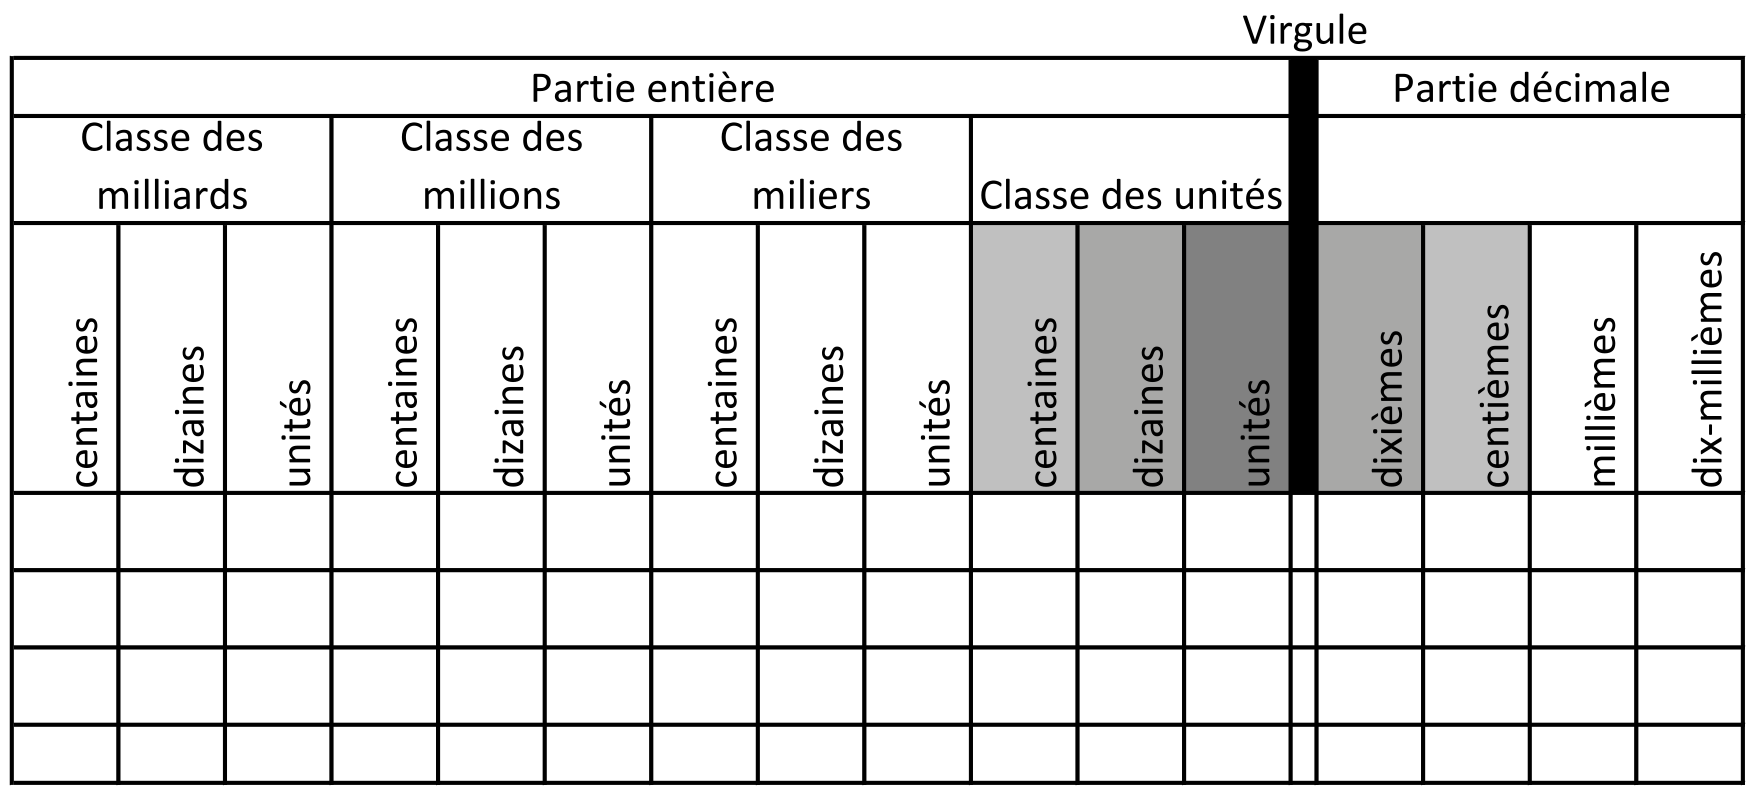
\includegraphics[scale=.18]{tab_rangs}\pause
	\end{center}

	\begin{exampleblock}{Exemples}
		\begin{itemize}
			\item \'Ecrire correctement le nombre 1845937126 : \pause
			
			Ce nombre s'écrit \num{1845937126}. \pause
			
			\item Donner la partie entière et la partie décimale de  \num{5239.67} :\pause
			La partie entière de \num{5239.67}  est \num{5239} et sa partie décimale est 67. \pause
			
			\item  Donner le chiffre des centaines et le nombre de dizaines de \num{1337}.\pause
			Dans \num{1337}, le chiffre des centaines est 3 et le nombre de dizaines est 133. \pause
				
			
			\item Donner une autre écriture possible du nombre 124 : \pause
			Le nombre \num{124} peut aussi s'écrire \num{124.00}.\pause
			
			%\item Le nombre \num{2048} est un nombre entier composé de 4 chiffres différents.
		\end{itemize}
	\end{exampleblock}
\end{frame}


\begin{frame}
	
	
	
	\begin{block}{Méthode}
		Pour \'ecrire un nombre en toutes lettres :\pause
		\begin{itemize}
			\item Tous les mots qui désignent un nombre sont invariables, sauf <<vingt>> et <<cent>>;\pause
			\item Les mots <<milliard>>, <<million>>, <<dixième>> ne désignent pas des nombres, ils prennent un <<s>> au pluriel;\pause
			\item 80 s'écrit <<quatre-vingts>> sauf s'il est suivi d'un autre nombre;\pause
			\item 100 s'écrit <<cents>> s'il est multiplié et non suivi d'un autre nombre, dans les autres cas il ne prend pas de <<s>>;\pause
			\item on écrit un trait d'union entre chaque mot d'un nombre.
		\end{itemize}
	\end{block}
\end{frame}

\begin{frame}
	\begin{exampleblock}{Exemples}
		\begin{itemize}
			\item 180 s'écrit \pause <<cent-quatre-vingts>>;\pause
			\item \num{1300} s'écrit \pause <<mille-trois-cents>>;\pause
			\item \num{4025035} s'écrit \pause <<quatre-millions-vingt-cinq-mille-trente-cinq>>;\pause
			\item \num{134.25} s'écrit \pause <<cent-trente-quatre unités vingt-cinq centièmes.
		\end{itemize}
	\end{exampleblock}
\end{frame}

%\section{Multiplier et diviser par 10, 100, 1000}
%
%\begin{frame}
%	\textbf{\underline{\textcolor{ForestGreen}{1) Multiplication}}}
%	
%	\begin{block}{Méthode}
%		Pour multiplier un nombre par 10, 100 ou 1000 :
%		\begin{enumerate}
%			\item on repère la virgule;
%			\item on la décale vers la droite d'un rang ($\times 10$) , de deux rangs ($\times 10$) ou de trois ($\times 10$);
%			\item on rajoute des zéros si besoin entre le chiffre le plus à droite et la virgule.
%		\end{enumerate}
%	\end{block}
%\end{frame}
%
%\begin{frame}
%	\begin{exampleblock}{Exemples}
%		\begin{itemize}
%			\item $\num{25.26} \times 10 = $
%			\item $\num{25.26} \times 100 = $
%			\item $\num{245.26} \times 1000 = $
%			\item $\num{285} \times 10 = $ 
%			\item $\num{285} \times 1000 = $ 
%		\end{itemize}
%	\end{exampleblock}
%\end{frame}
%
%
%\begin{frame}
%	\textbf{\underline{\textcolor{ForestGreen}{2) Division}}}
%	
%	\begin{block}{Méthode}
%		Pour diviser un nombre par 10, 100 ou 1000 :
%		\begin{enumerate}
%			\item on repère la virgule;
%			\item on la décale vers la gauche d'un rang ($\times 10$) , de deux rangs ($\times 10$) ou de trois ($\times 10$);
%			\item on rajoute des zéros si besoin entre la virgule et le chiffre le plus à gauche.
%		\end{enumerate}
%	\end{block}
%\end{frame}
%
%\begin{frame}
%	\begin{exampleblock}{Exemples}
%		\begin{itemize}
%			
%				\item $\num{25.26} \div 10 = $%\num{2.526}$ 
%				\item $\num{25.26} \div 1000 = $%\num{0.02526} $
%				\item $\num{245.26} \times 1000 = $% \num{245260}$
%				\item $\num{285} \div 10 = $%\num{28.5} $ 
%				\item $\num{285} \div 1000 = $%\num{0.285}$ 
%		
%		\end{itemize}
%	\end{exampleblock}
%\end{frame}
%
%\begin{frame}
%	\begin{alertblock}{Propriétés}
%		\begin{itemize}
%			\item Multiplier un nombre par \num{0.1}, \num{0.01} ou \num{0.001} revient à le diviser par 10, 100 ou 1000.
%			
%			\item Diviser un nombre par \num{0.1}, \num{0.01} ou \num{0.001} revient à le multiplier par 10, 100 ou 1000.
%		\end{itemize}
%	\end{alertblock}
%\end{frame}
%
%\begin{frame}
%	\begin{exampleblock}{Exemples}
%		\begin{itemize}
%			\item $\num{45.78} \times \num{0.1} = $%\num{45.78} \div \num{10} = \num{4.578}$ 
%			\item $\num{45.78} \times \num{0.01} = $%\num{45.78} \div \num{100} = \num{0.4578}$ 
%			\item $\num{45.78} \div \num{0.1} = $%\num{45.78} \times \num{10} = \num{457.8}$ 
%			\item $\num{45.78} \div \num{0.001} = $%\num{45.78} \times \num{1000} = \num{45780}$ 
%		\end{itemize}
%	\end{exampleblock}
%\end{frame}
%
%\section{Fractions décimales}

%\begin{frame}
%	\begin{enumerate}
%		\item Je convertis les fractions en nombre décimal :
%		
%		\begin{itemize}
%			\item $ \frac{3}{100} =$ \pause $ 3 \div 100 = \num{0.03}$ ;\pause
%			\item  $\frac{91}{100} = $ \pause $91 \div 100 = \num{0.91}$;\pause
%			\item $\frac{956}{100} = $ \pause $956 \div 100 = \num{9.56}$;\pause
%			\item $\frac{18}{1000} = $ \pause $18 \div 1000 = \num{0.018}$.
%		\end{itemize}
%		  
%		
%		J'additionne ces nombres aux temps et j'obtiens :
%		
%		{\footnotesize \begin{tabular}{|@{\ }c@{\ }|@{\ }c@{\ }|@{\ }c@{\ }|@{\ }c@{\ }|@{\ }c@{\ }|@{\ }c@{\ }|@{\ }c@{\ }|@{\ }c@{\ }|@{\ }c@{\ }|}
%			\hline
%			Appel à      & Léa         & Chloé       & Djamila      & Sarah        & Marine      & Sophiane    & Cindy        & Charlotte    \\ \hline
%			Temps (en s) & \num{19.98} & \num{20.03} & \num{29.690} & \num{19.893} & \num{19.91} & \num{28.56} & \num{20.018} & \num{19.935} \\ \hline
%		\end{tabular}}
%	
%	\vspace*{0.2cm}
%		
%		C'est donc avec Djamila qu'elle a passé le plus de temps et avec Sarah le moins.
%		
%		\item Je classe les appels téléphoniques du plus court au plus long :
%		
%		Sarah, Marine, Charlotte, Léa, Cindy, Chloé, Sophiane, Djamila.
%	\end{enumerate}
%\end{frame}
%
%\begin{frame}
%	\begin{mydef}
%		\begin{itemize}
%			\item Une \kword{fraction}, notée $\dfrac{n}{d}$ est une division entre deux nombres $n$ et $d$, séparés par un trait de fraction.
%			
%			\item $n$ est le \kword{numérateur} , $d$ est le \kword{dénominateur}.\pause
%		\end{itemize}
%		
%		
%		
%	\end{mydef}
%	
%	 \begin{exampleblock}{Exemple}
%	 	$\dfrac{15}{5}$ est une fraction.
%	 	
%	 	\begin{center}
%	 		\includegraphics<2>[scale=0.3]{frac1}
%	 		\includegraphics<3>[scale=0.3]{frac2}
%	 	\end{center}
%	 \end{exampleblock}
%\end{frame}
%
%\begin{frame}
%	\begin{alertblock}{Définitions}
%		\begin{itemize}
%			\item Une \kword{fraction décimale}, est une fraction où le dénominateur est un multiple de 10.		
%			
%			\item Toute fraction décimale peut s'écrire sous la forme d'un nombre décimal. C'est son \kword{écriture décimale}.\pause
%		\end{itemize}	
%	\end{alertblock}
%%
%	\begin{exampleblock}{Exemples}
%		\begin{itemize}
%			\item $\dfrac{145}{10}$ est une fraction décimale, son écriture décimale est \pause $\num{14.5}$.\pause
%			\item $\dfrac{72}{100}$ est une fraction décimale, son écriture décimale est \pause \num{0.72}.\pause
%			\item $\dfrac{9}{1000}$ est une fraction décimale, son écriture décimale \pause est \num{0.009}.
%		\end{itemize}
%	\end{exampleblock}
%%
%%
%\end{frame}






\section{Nombres et classement}


\begin{frame}
	\begin{alertblock}{Définitions}
	
			\begin{itemize}
				\item \kword{Comparer} des nombres, c'est dire si un est plus petit ou plus grand que l'autre ou s'ils sont égaux.\pause
				
				\item Ranger des nombres du plus petit au plus grand, c'est les classer par \kword{ordre croissant}.\pause
				
				\item Ranger des nombres du plus grand au plus petit, c'est les classer par \kword{ordre décroissant}.\pause
				
				\item \kword{Encadrer} un nombre, c'est trouver un nombre plus petit \textbf{et} un nombre plus grand que ce nombre.\pause
				
				\item \kword{Intercaler} un nombre entre deux autres, c'est un nombre compris entre ces deux nombres.
			\end{itemize}
			
	\end{alertblock}
\end{frame}

\begin{frame}
	\begin{myexs}
		\begin{itemize}
			\item 42 < 128, se lit \pause <<42 est inférieur à (ou plus petit que) 128>>;\pause
			\item 1337 < 1024, se lit \pause <<\num{1337} est supérieur à (ou plus grand que) \num{1024}>>;\pause
			\item 2 < \num{3.2} < \num{6.4} < \num{25.6} : ces nombres sont rangés dans l'ordre \pause croissant;\pause
			\item 123 > \num{45.6} > \num{7.89} > \num{5} : ces nombres sont rangés dans l'ordre \pause décroissant;\pause
			\item Encadrement de 21 à l'unité près : \pause 20 < 21 < 22 ;\pause
			\item Encadrement de \num{21.987} au centième près : \pause \num{21.977} < \num{21.987} < \num{21.997} ;\pause
		\end{itemize}
	\end{myexs}
\end{frame}


\begin{frame}
	\begin{myprop}
		Un point placé sur une demi-droite graduée est repéré par un nombre, son \kword{abscisse}.
	\end{myprop}
	
	\begin{myex}
		\begin{center}
			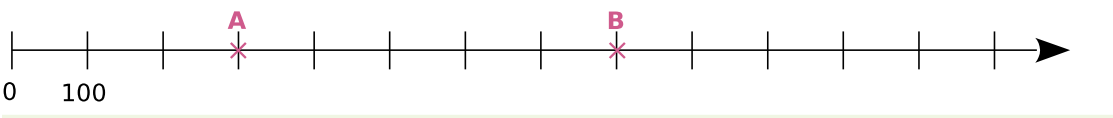
\includegraphics[scale=0.4]{../img/axe}
		\end{center}
		
		\begin{itemize}
			\item L'abscisse du point A est :
			\item L'abscisse du point B est :
			\item L'abscisse du point C est : 500;
			\item L'abscisse du point D est \num{1100}.
		\end{itemize}
	\end{myex}
\end{frame}
\end{document}